\documentclass[aps, prb, twocolumn, a4paper, floatfix, reprint]{revtex4-2}
\usepackage[%
    margin=10mm,% ако не си принтира 10мм не изглежда грозно, а може да събереш повече текст
    % showframe=true,%
    ]{geometry}
\usepackage[T1,T2A]{fontenc}
\usepackage[utf8]{inputenc}
\usepackage[main=bulgarian, english]{babel}
\usepackage{float}
\AtBeginDocument{\selectlanguage{bulgarian}}
\newcommand{\degree}{^{\circ}}
\usepackage{amsmath}
\usepackage{graphics}
\usepackage{graphicx}
\graphicspath{{.}}
\newcommand{\abs}[1]{\lvert#1\rvert}
\let\phi\varphi
\usepackage{booktabs} % от тук се използва само \midrule може и без него 
%\usepackage{adjustbox} % това може да се използва, за да „смаляваш“ широки таблици
%\usepackage{tabularx} % дефинира колона X в среда tabularx която добавя празно място така че цялата таблица да запълни определена ширина
\usepackage{dcolumn}
\newcolumntype{d}[1]{D{.}{.}{#1}}
\usepackage[unicode=true,pdfusetitle]{hyperref}


\makeatletter
\renewcommand{\Dated@name}{}%
\makeatother



\begin{document}
\title{Стробоскопичен ефект}
\author{Васил Николов}
\noaffiliation
\date{21.11.2021}
\maketitle

\section{Цел на упражнението}
Да се изследва праволинейно и криволинейно движение на тяло, което записва положението си върху лист хартия с дадена честота $(f=100Hz)$

\section{Експериментална установка}
Пишещата глава е малка пластмасофа кутия, на дъното на която има чукче. Когато на кутията се пусне напрежение чукчето започва да трепти с честота $(f=100Hz)$. Когато пишещото устройство се постави върху лист индиго, а той се постави върху нормален лист хартия устройството "записва" положението си върху листа под формата на мастилени точки. Чрез анализ на разстоянието между поредните точки може да се намерят средната скорост и ускорение във всяка точка от кривата. 

\section{Теоретична обосновка}
Нека $\vec{r}_i$ е радиусвекторът на точка с пореден номер $i$, а $\Delta t = 1/f$ е времевият интервал между две точки. Тогава средната скорост и средното ускорение на тялото в точка $i$ е 
\begin{subequations} \label{eq:1} 
\begin{gather} 
    \vec{v_i} = \frac{\vec{r}_{i + 1} - \vec{r}_{i - 1}}{2\Delta t} \\
    \vec{a_i} = \frac{\vec{v}_{i + 1} - \vec{v}_{i - 1}}{2\Delta t} 
\end{gather}
\end{subequations}

\section{Обработка на данните}
Листът, на който са точките се снима, и дигитално се снемат коордитатите на точките в пиксели. На листа се нанася и мащаб - отсечка, чиято дължина знаем. Като се снемат краищата на отсечката като още две точки може да се определи мащабът на снимката, и да се пресметне на какви координати в сантиметри отговарят координатите в пиксели. След това по формулите, описани в \eqref{eq:1} се пресмятат векторите на ускорението и скоростта. На снимката се нанасят вектори с начало избраните точки с дължина, пропорционална на съответно скоростта и ускорението. За целта се избира такъв мащаб, че стрелките да не се припокриват много, но и да не са твърде къси. 

\section{Експериментални данни и резултати}

На фигурата с червени стрелки е скоростта на главата, а със сини - ускорението й. Посоките на скоростта и ускорението във всяка точка съвпадат с очакванията ни.
\begin{figure}[h]
    \caption{Скорост и ускорение при криволинейно движение}
    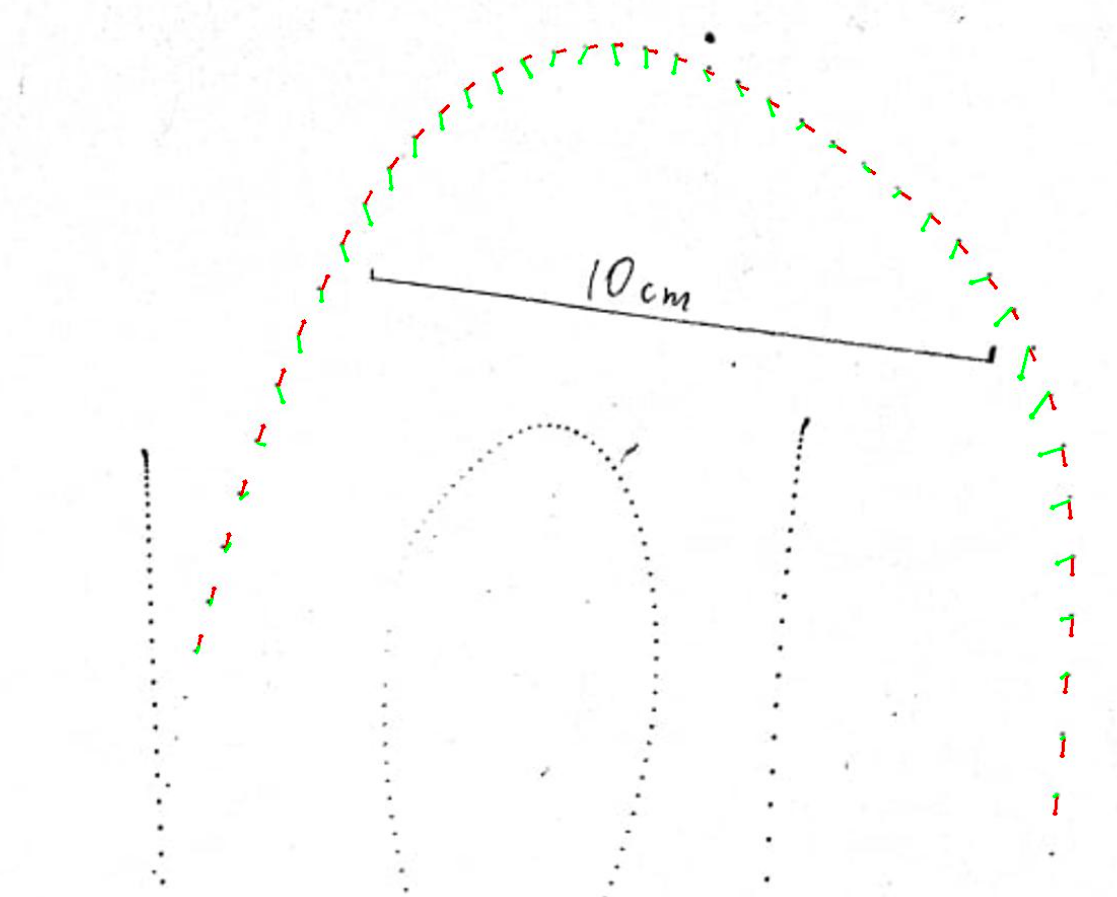
\includegraphics[width=0.9\columnwidth,keepaspectratio=true]{cropped_velocity_acceleration.png}
\end{figure}

\begin{figure}[H]
    \caption{Скорост при праволинейно движение на тялото}
    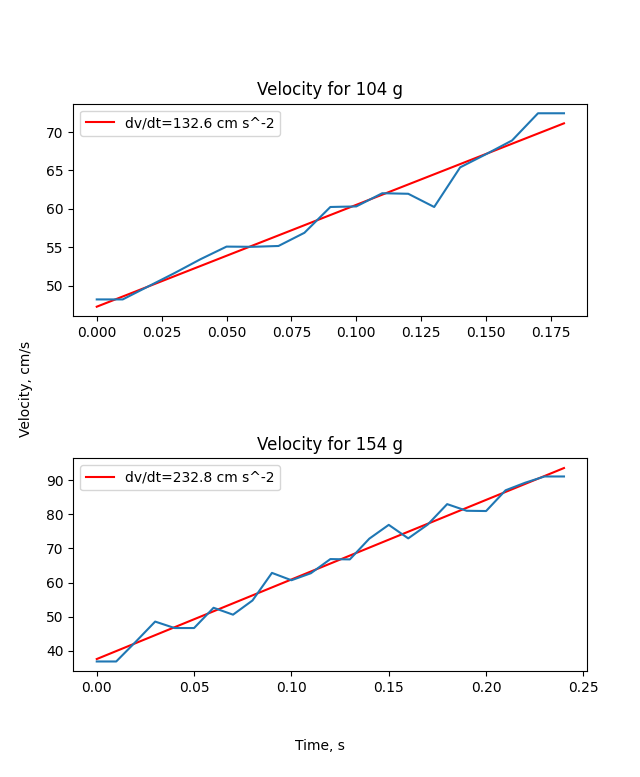
\includegraphics[width=0.9\columnwidth,keepaspectratio=true]{vel_charts_3.png}
\end{figure}

На двете графики са дадени скоростта и ускорението на тялото когато се дърпа от съответно $104 g$ и $154 g$. При снемане на позиции на точките, особено когато разстоянието между тях е малко, се натрупва голяма грешка при измерване, заради която графиката не е идеална права, и пресметнатото ускорение не е близко до очакваното постоянно ускорение. Заради това графика на ускоренията от времето не са представени. 


\end{document}